\documentclass[a4paper]{article}

\usepackage[english]{babel}
\usepackage[T1]{fontenc}  			% make sure to install cm-super package for improved PDF quality
\usepackage[utf8]{inputenc}
%\usepackage[cm]{fullpage}			% Fullpage for now
\usepackage{graphicx}
\usepackage[dvipsnames]{xcolor}
\usepackage[font=small]{caption}
\usepackage{subcaption}
\usepackage{microtype}			 	% microtypographical fine-tunning
\usepackage{setspace} 				% Provides support for setting the spacing between lines in a document.
\usepackage{tocbibind}				% Add bibliography/index/contents to Table of Contents.
\usepackage{mathtools}				% enhances amsmath (no need to load amsmath)
\usepackage{amssymb}
\usepackage{amsfonts}
\usepackage{amsthm}
\usepackage{bm} 					% bold math symbols including greek letters
\usepackage{booktabs}				% professional tables (w/o vertical bars)
\usepackage{array}					% 
\usepackage{dcolumn} 				% align to decimal point in tables
\usepackage[shortcuts]{extdash} 	% hyphenation of dashed words
\usepackage[algoruled]{algorithm2e}
\newcommand\mycommfont[1]{\small\ttfamily #1}
\SetCommentSty{mycommfont}
\usepackage{cleveref}				% clever environment referencing
\crefname{figure}{Fig.}{Figs.}
\crefname{algorithm}{Alg.}{Algs.}
\usepackage{siunitx}				% typesetting of SI units
%\usepackage{paralist}		     	% compact lists with more options
%\usepackage[]{todonotes}			% TODO notes
%\presetkeys{todonotes}{backgroundcolor=orange!50}{}
% Not sure which to use for bibliography
%\usepackage{cite}
%\usepackage{citesort}
\usepackage[square, sort, numbers, authoryear]{natbib}
\usepackage{pgfplots}


\begin{document}

\section{Euler's Method}\label{sec:euler_method}
It's the simplest method of numerical solution for ordinary differential equations (ODEs).
Suppose we are given the following ODE with and initial condition
\begin{equation}\label{eq:ode}
	y'(t) = f(t, y(t)), \quad y(t_0) = y_0,
\end{equation}
where \( y'(t) = \frac{\mathrm{d}y}{\mathrm{d}t} \) denotes derivative.
Derivatives with respect to time, which are common in physics, are conventionally denoted by the dot symbol. 
That is \( \dot{y}(t) \equiv y'(t) \equiv \frac{\mathrm{d}y}{\mathrm{d}t} \).
\Cref{eq:ode} is in continuous time \( t \)\footnote{Since this is mathematics we're dealing with, the variable \( t \) does not have to represent time, of course.}.
To solution of the ODE above is a function of time \( y(t) \) for which the above equation holds.
Since we are working with computers, we can't store functions of continuous variable\footnote{Because that would take up infinite memory.} and so we need to discretize the solution.
In other words, we wanna convert it to an equation in discrete time, because it's easier to implement.

The Euler method chooses some finite time step \( h \), so that \( k \)-th discrete time step can be expressed as \( t_k = t_0 + kh \).
One step of the Euler method from \( t_k \) to \( t_{k+1}  = t_k + h \) is given by
\begin{equation}
	y_{k+1} = y_k + hf(t_k, y_k),
\end{equation}
where, obviously, \( y_k = y(t_k) \).
As you can see, the recursion can be started with \( y_0 \) at \( t_0 \), because both of these are given.
We can rewrite the Euler method as 
\begin{equation}
	\frac{y_{k+1} - y_k}{h} = f(t_k, y_k)
\end{equation}

So, for example if my equation for the change in the x-coordinate in the continuous time is given by
\begin{equation}
	\dot{x}(t) = v(t)\cos(\psi(t)),
\end{equation}
than, by application of the Euler method, the discretized version with step size \( h = \mathrm{d}t \) will look like this
\begin{equation}\label{}
	x(t_{k+1}) = x(t_{k}) + v(t_k)\cos(\psi(t_k)) \mathrm{d}t.
\end{equation}
Now, to comport with the notational conventions, we are gonna use the lower index to denote the discre time steps. Since the time steps are only distinguished by the variable \( k \), using variable \( t \) is a bit redundant (so we will get rid of it too).
Ultimately, we get
\begin{equation}\label{eq:ode_euler}
	x_{k+1} = x_{k} + v_k\cos(\psi_k) \mathrm{d}t.
\end{equation}

With the help of the Euler method, we have converted a \emph{differential} equation into a \emph{difference} equation.
There are plenty of other, more accurate, methods for ODE integration, such as Runge-Kuta method (see Wikipedia for more), but they are more complicated.



\section{Kinematic Bicycle Model}\label{sec:kinematic_bicycle_model}
This is the kinematic bicycle model
\begin{align}\label{eq:kinematic_bicycle_model_continuous}
	\dot{x} 	&=  v \cos(\psi + \beta) \\
	\dot{y} 	&=  v \sin(\psi + \beta) \\
	\dot{\psi} 	&=  \frac{v}{l_r} \sin(\beta) \\
	\dot{v} 	&=  a \\
	\dot{\beta} &= \arctan\left(\frac{l_r}{l_r + l_f}\tan(\delta_f)\right)
\end{align}
The \Cref{fig:kinematic_bicycle_model}, stolen from \cite{Kong2015}, depicts the geometric meaning of the variables involved.
\begin{figure}[h]
	\centering
	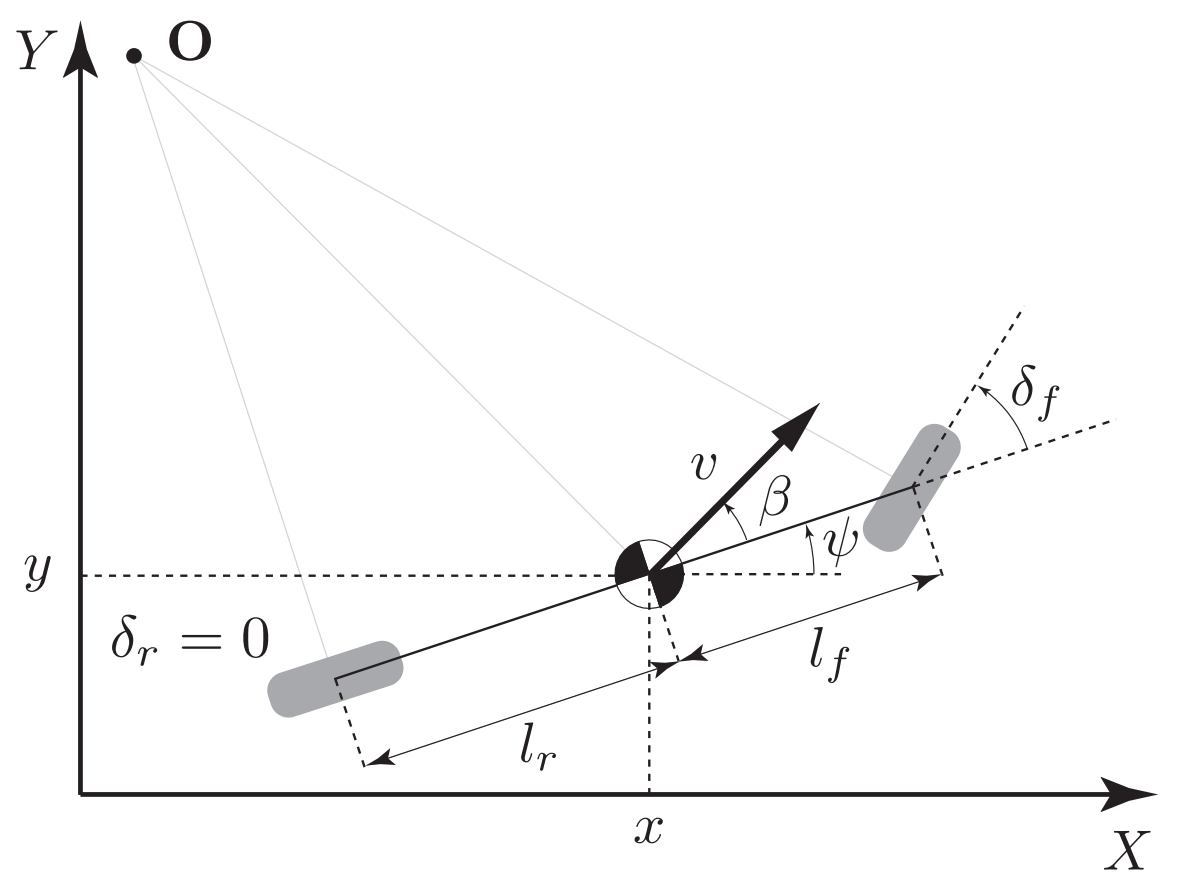
\includegraphics[scale=0.2]{./img/kinematic_bicycle_model.png}
	\caption{Kinematic bicycle model.}
	\label{fig:kinematic_bicycle_model}
\end{figure}

For some undisclosed reason, at Udacity, we are using a simplified version, given by
\begin{align}\label{eq:kinematic_bicycle_model_continuous_udacity}
\dot{x} 	&=  v \cos(\psi) \\
\dot{y} 	&=  v \sin(\psi) \\
\dot{\psi} 	&=  \frac{v}{l_r} \delta_f \\
\dot{v} 	&=  a \\
\end{align}
Applying the Euler method from \Cref{sec:euler_method} yields the familiar equations
\begin{align}\label{eq:kinematic_bicycle_model_discrete_udacity}
x_{k+1} 	&= x_k + v_k\cos(\psi_k) \mathrm{d}t \\
y_{k+1} 	&= y_k + v_k\sin(\psi_k) \mathrm{d}t \\
\psi_{k+1} 	&= \psi_k + \frac{v_k}{l_r}\delta_f \mathrm{d}t \\
v_{k+1} 	&= v_k + a_k*\mathrm{d}t \\
\end{align}
where the \( \mathrm{d}t \) is the discretization step size.




\section{Model Predictive Control}\label{sec:model_predictive_control}




% ==========================
\bibliographystyle{plainnat}
\bibliography{refereces}

\end{document}